% \documentclass[a4paper,10pt]{article}
\documentclass[review]{siamart}
\usepackage{url}
\usepackage{amssymb}
\usepackage{amsmath}
\usepackage{bm}
\usepackage{stmaryrd}
\usepackage{array}
\usepackage{empheq}
\usepackage{enumitem}
	\setlist{nosep} % or \setlist{noitemsep} to leave space around whole list
\usepackage{color}
%\usepackage{showlabels}
\usepackage{adjustbox}
\usepackage{hyperref}
\hypersetup{
  colorlinks   = true, %Colours links instead of ugly boxes
  urlcolor     = blue, %Colour for external hyperlinks
  linkcolor    = blue, %Colour of internal links
  citecolor   = red %Colour of citations
}
\usepackage[numbers,sort]{natbib}
\usepackage{cleveref}

\newsiamremark{remark}{Remark}


% \newtheorem{lemma}{Lemma}
% \newtheorem{definition}{Definition}
% \newtheorem{theorem}{Theorem}
% \newtheorem{corollary}{Corollary}

\newcommand{\tcb}{\textcolor{blue}}
\newcommand{\tcp}{\textcolor{purple}}
\newcommand{\todo}[1]{\textcolor{red}{[TODO\@: #1]}}

\newcommand{\mdet}{\operatorname{det}}
\newcommand{\madj}{\operatorname{adj}}

% ------------------------------------------------------------------------------------ %
% ------------------------------------------------------------------------------------ %

\newcommand{\TheTitle}{IRK!}
\newcommand{\TheAuthors}{B.S. Southworth }
\headers{IRK!}{\TheAuthors}
\title{{\TheTitle}\thanks{This research was conducted ...
  }}

\author{%
  Ben~S.~Southworth
  \thanks{Department of Applied Mathematics,
          University of Colorado at Boulder
          (\email{ben.s.southworth@gmail.com}).}
}

\ifpdf%
\hypersetup{%
  pdftitle={\TheTitle},
  pdfauthor={\TheAuthors}
}
\fi

% ------------------------------------------------------------------------------------ %
% ------------------------------------------------------------------------------------ %

\begin{document}
\allowdisplaybreaks



% ------------------------------------------------------------------------------------ %
% ------------------------------------------------------------------------------------ %
\section{Implementation details}

The basic idea is that at each time step, we need to update the previous solution with
\begin{align} \label{eq:RK_update}
\bm{u}_{n+1}  = \bm{u}_n + \delta t \mdet({\cal M}_s)^{-1} \big( \bm{d}^\top_0 \otimes I \big) \madj({\cal M}_s) \big( I \otimes M^{-1} \big) \bm{f},
\end{align}
where we have
\begin{itemize}
\item $m \in \mathbb{N}$: The dimension of the spatial problem

\item $\bm{f} = (\bm{f}_1, \ldots, \bm{f}_s)^\top$, with $\bm{f}_j = {\cal L} \bm{u}_n + \bm{g}(t_n + c_j \delta t) \in \mathbb{R}^m$

\item $\bm{d}_0 \coloneqq A^{-\top}_0 \bm{b}_0 \in \mathbb{R}^{s}$ 

\item $M \in \mathbb{R}^{m \times m}$ is the mass matrix
\end{itemize}

Now we break \eqref{eq:RK_update} into two steps:
\begin{enumerate}
\item{Step 1:}\label{it:update_step1} Compute 
\begin{align} \label{eq:step1}
\bm{z} = \big( \bm{d}^\top_0 \otimes I \big) \madj ({\cal M}_s) \big(I \otimes M^{-1} \big)\bm{f} \in \mathbb{R}^m
\end{align}

\item{Step 2:}\label{it:update_step2} Solve
\begin{align} \label{eq:step2}
\mdet( {\cal M}_s ) \bm{y} = \bm{z},
\end{align}
then update per \eqref{eq:RK_update}, $\bm{u}_{n+1} = \bm{u}_n + \delta t \bm{y}$
\end{enumerate}

Note that problem arises from solving the linear system for $(A_0 \otimes I_m) \bm{k}$
\begin{align}
{\cal M}_s (A_0 \otimes I_m) \bm{k} = (I_s \otimes M^{-1}) \bm{f}, 
\quad 
{\cal M}_s \coloneqq A_0^{-1} \otimes I_m - I_s \otimes \delta t M^{-1} {\cal L}.
\end{align}


% ------------------------------------------------------------------------------------ %
% ------------------------------------------------------------------------------------ %
% ------------------------------------------------------------------------------------ 
\subsection{On Step \ref{it:update_step1}}

$\madj ({\cal M}_s)$ is defined by evaluating the adjugate of $A_0^{-1} - zI$ at $z = \delta t \widehat{\cal L}$, where $\tcb{\widehat{\cal L} \coloneqq M^{-1} {\cal L}}$, which is a matrix over polynomials of degree $s-1$ in $z$. If we write such polynomials as $Q_{ij}(z) \coloneqq \madj(A_0^{-1} - zI)_{ij}$, then
\begin{align}
\madj ({\cal M}_s) = 
\begin{bmatrix}
Q_{11}(\delta t \widehat{\cal L}) & \cdots & Q_{1s}(\delta t \widehat{\cal L}) \\
\vdots & & \vdots \\
Q_{s1}(\delta t \widehat{\cal L}) & \cdots & Q_{ss}(\delta t \widehat{\cal L})
\end{bmatrix}
\in \mathbb{R}^{ms \times ms},
\quad
Q_{ij}({\cal L}) = \sum \limits_{k = 0}^{s-1} \hat{q}_{ijk} {\cal L}^k \in \mathbb{R}^{m \times m}.
\end{align}
For sensible $s \in \mathbb{N}$, we can symbolically compute $\madj(A_0^{-1} - zI)$ in terms of an arbitrary matrix $A_0^{-1}$, and, thus, we can compute the sets of coefficients $\{ \hat{q}_{ijk} \}_{(i,j,k)=(1,1,0)}^{(s,s,s-1)}$.

Now, the rectangular Kronecker product matrix appearing in front of this matrix simply takes inner products over its columns to give a block rectangular matrix whose elements are therefore polynomials in $\widehat{\cal L}$ of degree $s-1$:
\begin{align}
\big( \bm{d}_0^\top \otimes I \big) \madj({\cal M}_s) 
=
\begin{bmatrix}
X_{1}(\delta t \widehat{\cal L}), \, \cdots, \, X_{s}(\delta t \widehat{\cal L})
\end{bmatrix},
\end{align}
where
\begin{align}
X_{j}({\cal L}) = \sum \limits_{k = 0}^{s-1} \hat{x}_{j k} {\cal L}^k \in \mathbb{R}^{m \times m}, 
\quad
\hat{x}_{j k} = \sum \limits_{\ell = 1}^s d_{0,\ell} \, \hat{q}_{\ell j k}.
\end{align}
Using the coefficients $\{ \hat{q}_{ijk} \}_{(i,j,k)=(1,1,0)}^{(s,s,s-1)}$ we can compute the coefficients $\{ \hat{x}_{jk} \}_{(j,k)=(1,0)}^{(s,s-1)}$, which are the things we actually need (that is, we don't need the intermediate $\hat{q}_{ijk}$). Thus, in the implementation, we have coefficients $\{ \hat{x}_{jk} \}_{(j,k)=(1,0)}^{(s,s-1)}$ implemented symbolically in terms of general $\bm{d}_0$ and $A_0^{-1}$ for sensible values of $s$. When the user specifies a particular Butcher tableaux (and hence a specific $s$), the appropriate set of coefficients are evaluated numerically and stored in memory so that the polynomials $\{X_{j}(\delta t \widehat{\cal L})\}$, can be evaluated as needed by the algorithm.

Finally, the vector in \eqref{eq:step1} can be written as the sum
\begin{align} \label{eq:z_sum}
\bm{z} = \sum \limits_{i = 1}^s [X_i(\delta t \widehat{\cal L})] (M^{-1} \bm{f}_i).
\end{align}
The main task here is computing the action of the degree $s-1$ polynomials $\{X_j(\delta t \widehat{\cal L})\}$ on the components $M^{-1} \bm{f}_i$.  \tcp{Ben: It's not true in general that $M^{-1}$ will commute with a monomial in $M^{-1} {\cal L}$, is it? So we have to do this mass matrix solve in the eqn. above on every component of $\bm{f}$ rather than pulling this $M^{-1}$ out the front of the entire sum?} \tcb{Yes. But if $\bm{f}_j = {\cal L} \bm{u}_n + \bm{g}(t_n + c_j \delta t)$,
applying $M^{-1}$ to this equation is the same as the Mult() function in MFEM I believe, which the user has to
implement in time dependent operator. If the forcing function $\mathbf{g}$ is indepenent of time, we could just
compute once, although it's really not that much work to do it once for each stage.}
I think the most efficient way to compute the action of such polynomials is with a Horner-like scheme, which is a well-known technique for evaluating scalar polynomials (see \url{https://en.wikipedia.org/wiki/Horner\%27s_method}). Basically, we can compute the action of the $n$th degree polynomial $P_n({\cal L})$ on a vector using: $n$ \texttt{MATVECs} with ${\cal L}$, $n+1$ \texttt{AXPYs} ($\bm{x} \gets \alpha \bm{y} + \beta \bm{z}$), $n$ \texttt{copies} ($n$ lots of copying values from one vector to another, $n \times [\bm{x} \gets \bm{y}]$), and one intermediate/temporary vector. Thus, the main cost in computing \eqref{eq:z_sum} is $s(s-1)$ \texttt{MATVECs} with $\widehat{\cal L} = M^{-1} {\cal L}$, and a secondary cost is the $s$ actions of $M^{-1}$ on the vectors $\{\bm{f}_j\}_{j = 1}^s$.



% ------------------------------------------------------------------------------------ %
% ------------------------------------------------------------------------------------ %
% ------------------------------------------------------------------------------------ 
\subsection{On Step \ref{it:update_step2}}
As shown previously, 
\begin{align}
\mdet ({\cal M}_s) = P_s(\delta t \widehat{\cal L}) = \prod \limits_{j = 1}^s (\lambda_j I - \delta t \widehat{\cal L}),
\end{align}
where $\{ \lambda_j \}_{j = 1}^s$ are the eigenvalues of $A_0^{-1}$. Now we're going to split the eigenvalues into two disjoint subsets based on their being real and complex:
\begin{align}
\{\lambda_j \}_{j = 1}^s = \{\zeta_j \}_{j = 1}^{s_{\Re}} \cup \{ \eta_j + \imath \beta_j, \eta_j - \imath \beta_j \}_{j = 1}^{s_{\Im}}, 
\quad \eta_j, \beta_j, \zeta_j \in \mathbb{R},
\quad s = s_{\Re} + 2 s_{\Im}.
\end{align}
That is, $\{\zeta_j \}_{j = 1}^{s_{\Re}}$ are the $0 \leq n_{\Re} \leq s$ real eigenvalues of $A_0^{-1}$, and $\{ \eta_{j} + \imath \beta_{j}, \eta_{j} - \imath \beta_{j} \}_{j = 1}^{s_{\Im}}$ are the $0 \leq {n_{\Im}} \leq \left \lfloor{s/2}\right \rfloor $ complex, conjugate-pair, eigenvalues of $A_0^{-1}$. 

To invert characteristic polynomial $P_s$, we do so by inverting only real factors. This means that complex-conjugate pairs are combined to become quadratic polynomials in ${\cal L}$. That is, we have
\begin{align} 
P_s (\delta t \widehat{\cal L}) 
&= 
\prod \limits_{j = 1}^{s_{\Re}} {\cal R}_j(\delta t \widehat{\cal L}) \prod \limits_{j = 1}^{s_{\Im}} {\cal I}_j(\delta t \widehat{\cal L}),\\
\quad 
{\cal R}_j(\delta t \widehat{\cal L}) 
&\coloneqq 
\zeta_j I - \delta t \widehat{\cal L}, \\
{\cal I}_j(\delta t \widehat{\cal L})
&\coloneqq
[\eta_j^2 + \beta_j^2] I - 2 \eta_j \delta t \widehat{\cal L} + (\delta t \widehat{\cal L})^2.
\end{align}
\begin{enumerate}
\item \textbf{Linear factors:} To solve the system 
\begin{align}
{\cal R}_j(\delta t \widehat{\cal L}) \bm{y}_j = (\zeta_j I -  \delta t M^{-1} {\cal L}) \bm{y}_j = \bm{z}_j,
\end{align}
we first scale both sides of the problem by ${M}$ to give
\begin{align}
(\zeta_j M -  \delta t {\cal L}) \bm{y}_j = M \bm{z}_j.
\end{align}
This system is then solved by GMRES (or CG/MINRES if ${\cal L}$ is symmetric) which is preconditioned by a single iteration of AMG applied to the matrix $(\zeta_j M -  \delta t {\cal L})$. So, per Krylov iteration, the action of $M$ is required once. Note that not scaling the system and applying an AMG preconditioner to the sparse matrix $(\zeta_j M -  \delta t {\cal L})$ requires the action of both $M$ and $M^{-1}$ every Krylov iteration.

\item \textbf{Quadratic factors:} To solve the system
\begin{align}
{\cal I}_j(\delta t \widehat{\cal L}) \bm{y}_j 
=
\big( [\eta_j^2 + \beta_j^2] I - 2 \eta_j \delta t M^{-1} {\cal L} + (\delta t M^{-1} {\cal L})^2 \big) \bm{y}_j
= \bm{z}_j,
\end{align}
we first scale both sides by $M$ to give
\begin{align}
\big( [\eta_j^2 + \beta_j^2] M - 2 \eta_j \delta t {\cal L} + \delta t^2 {\cal L} M^{-1} {\cal L} \big) \bm{y}_j
= M \bm{z}_j.
\end{align}
This system is then solved by GMRES (or CG/MINRES if ${\cal L}$ is symmetric; note the operator is symmetric in this instance \tcb{(but is it SPD?)}) which is preconditioned by \underline{twice} applying a \textit{small}, fixed number of iterations (likely one) of AMG to the matrix $(\eta_j M -  \delta t {\cal L})$; however, before the second application of AMG, the RHS needs to be scaled by $M$.\footnote{To see why this is true, say $\beta_j = 0$, then the system we'd be solving is $(\eta_j M - \delta t {\cal L}) (\eta_j I - \delta t M^{-1} {\cal L}) \bm{y}_j = M \bm{z}_j$, and, so, when we come to precondition this system by twice inverting $\eta_j M - \delta t L$, we can invert it once to solve the system $(\eta_j M - \delta t L) \hat{\bm{y}}_j =  M \bm{z}_j$, where $\hat{\bm{y}}_j = (\eta_j I - \delta t M^{-1} {\cal L}) \bm{y}_j$. But before we can solve $(\eta_j I - \delta t M^{-1} L) \bm{y}_j = \hat{\bm{y}}_j$ by inverting $(\eta_j M - \delta t L)$, we must first scale the system by $M$.} So, per Krylov iteration, the action of $M^{-1}$ is required once, and the action of $M$ twice. Note that if the system were not scaled originally by $M$, then the action of $M$ and $M^{-1}$ would be required twice each per Krylov iteration ($M^{-1}$ in the action of the operator, and $M$ to scale the right hand sides in the preconditioner).
\end{enumerate}


\tcp{Ben: So why cant we approximately invert $(\eta_j M - \delta t {\cal L})$ with GMRES preconditioned by AMG? You mentioned in the code I'd written that this doesn't work. My thinking was that we need to approximately invert $(\eta_j M - \delta t {\cal L})$ and GMRES preconditioned with AMG will do this more robustly than standalone AMG?}
{\color{blue}
GMRES forms an optimal linear combination over a Krylov space. The $k$th Krylov space takes the form of powers
of the preconditioned operator times an initial residual, $\mathcal{K} := \{\mathbf{r}_0, (M^{-1}A)\mathbf{r}_0, 
..., (M^{-1}A)^k\mathbf{r}_0\}$. This results in an approximation to the linear system given by a polynomial
in the preconditioned operator. For this to make sense, it is important that every time you take a further
GMRES iteration, which computes a new power, $(M^{-1}A)^k\mathbf{r}_0$, that you use the same $M^{-1}$ as in
previous iterations. Now suppose $M^{-1}$ actually corresponds to an inner GMRES approximation. Then every
outer GMRES iteration has a different right-hand side, and the result is that the inner GMRES approximate 
inverse is a different polynomial for every outer iteration. This means you are using a different preconditioner
for every iteration, and GMRES will be very unhappy.

Flexible GMRES is a GMRES-like algorithm that allows for different preconditioners each iteration. This would
work with what you are talking about, but also doesn't make sense here. Because full memory GMRES is already
optimal, it doesn't make sense to try to optimize the inner solve. You're always going to be taking a polynomial
in the preconditioned operator. If you use only outer GMRES, then every application of the AMG preconditioner is 
made to be optimal with respect to the larger quadratic linear system. If you use inner GMRES for, say, 10
iterations,  those 10 AMG applications are made optimal to approximate the inverse of the inner linear system,
but this is probably not optimal to solve the larger quadratic operator. Often in situations like this, you
actually gain very little improvement in convergence by applying more iterations to an inner linear system.
}


% ------------------------------------------------------------------------------------ %
% ------------------------------------------------------------------------------------ %
% ------------------------------------------------------------------------------------ 
\newpage
\section{Numerical results}

Numerically approximate the solution of the 2D, constant-coefficient advection-diffusion problem,
\begin{align}
u_t + 0.85 u_x + 1.0 u_y = 0.3 u_{xx} + 0.25 u_{yy}  + s(x,y,t),
\quad (x,y,t) \in  (-1,1)^2 \times (0, 2)
\end{align}
Some remarks:
\begin{itemize}
\setlength\itemsep{0.5em}
\item Periodic spatial boundaries. All tests use 4 processors.

\item A $p$th-order IRK scheme is coupled with $p$th-order central finite differences in space (or $p$+1st-order if $p$ is odd, as for Radau IIA and some SDIRK schemes).

\item Set $\delta t = 2 \delta x$

\item Tests in Figure \ref{fig:errors2D} indicate that the code is implemented and working properly since theoretically predicated convergence rates are obtained in all cases.

\item GMRES: \texttt{abs tol=rel tol=1e-13}

\item From Figure \ref{fig:errors2D}, Gauss and Radau appear scalable with respect to problem size. Noting that the grid complexities for all of the AMG solves seem comparable (for the 4th-order schemes they're around 1.7), Gauss certainly seems like it requires the least amount of work.

\item \tcp{Note that obtaining these kind of scalable iteration counts for the non-SDIRK schemes is dependent on the AMG preconditioner doing a good enough job. I've made some comments in the top of \texttt{IRK\_lin\_class/driver\_adv\_dif\_FD.cpp} about this. But essentially with the current setup, adding a single level of aggressive coarsening destroys this scalability, and we instead see GMRES/AMG iteration counts increase significantly Gauss, Radau, Lobatto. However, with even with aggressive coarsening, GMRES/AMG iterations remain fixed for SDIRK iteration... So I'm not really sure that the results in Figure \ref{fig:iters2D} are a fair comparison given that the  AMG solvers for SDIRK can be made significantly cheaper...}

\end{itemize}


\begin{figure}[H]
\centerline{
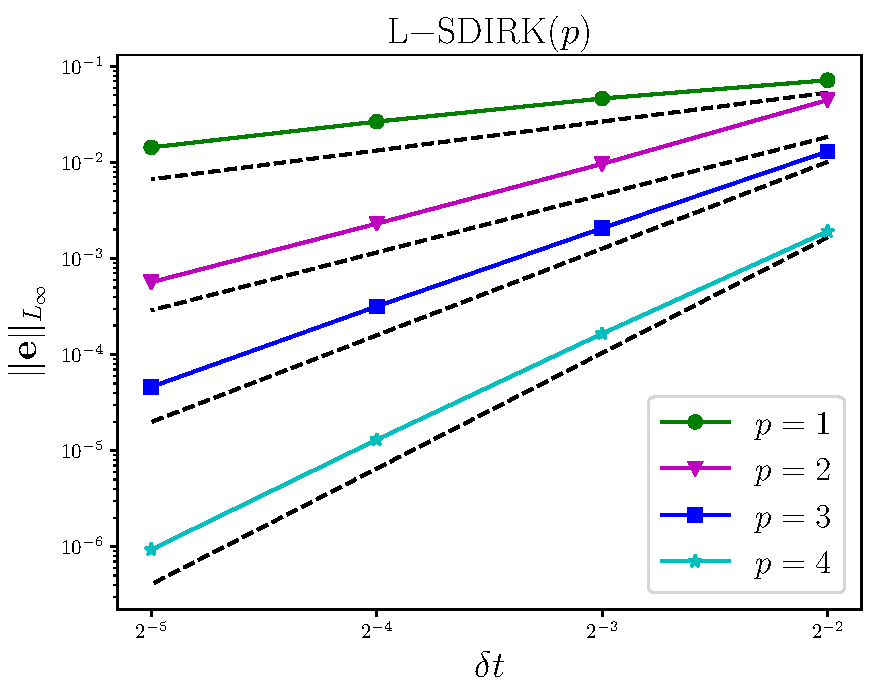
\includegraphics[width = 0.55\textwidth]{figures/LSDIRK_d2_ex1.pdf}
\quad
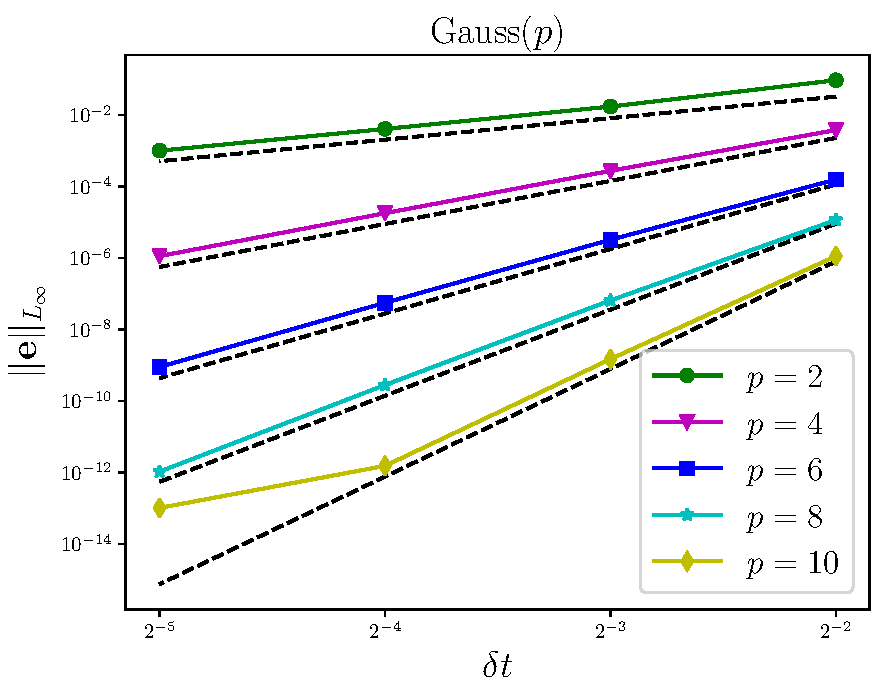
\includegraphics[width = 0.55\textwidth]{figures/Gauss_d2_ex1.pdf}
}
\centerline{
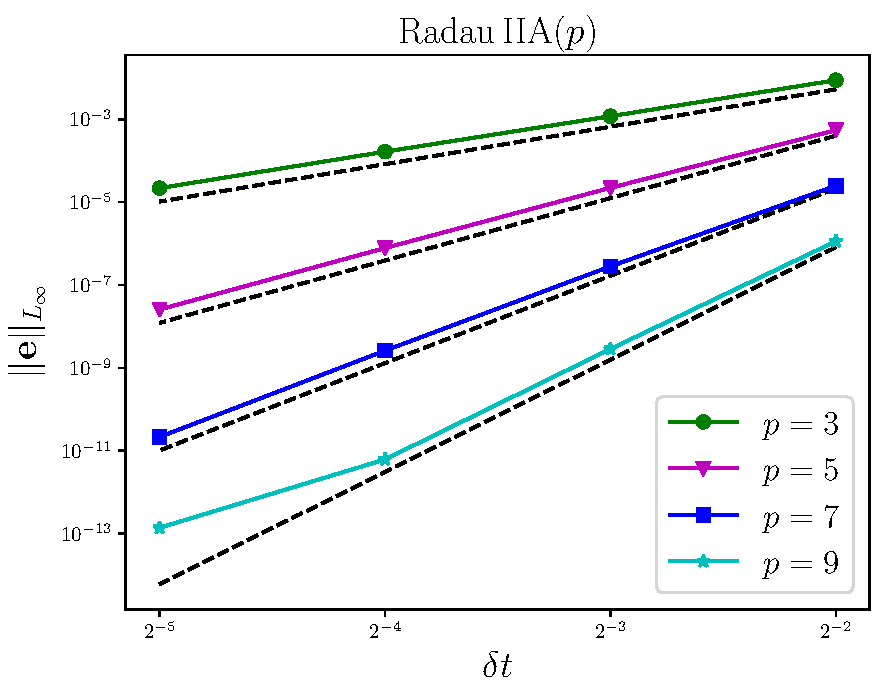
\includegraphics[width = 0.55\textwidth]{figures/RadauIIA_d2_ex1.pdf}
\quad
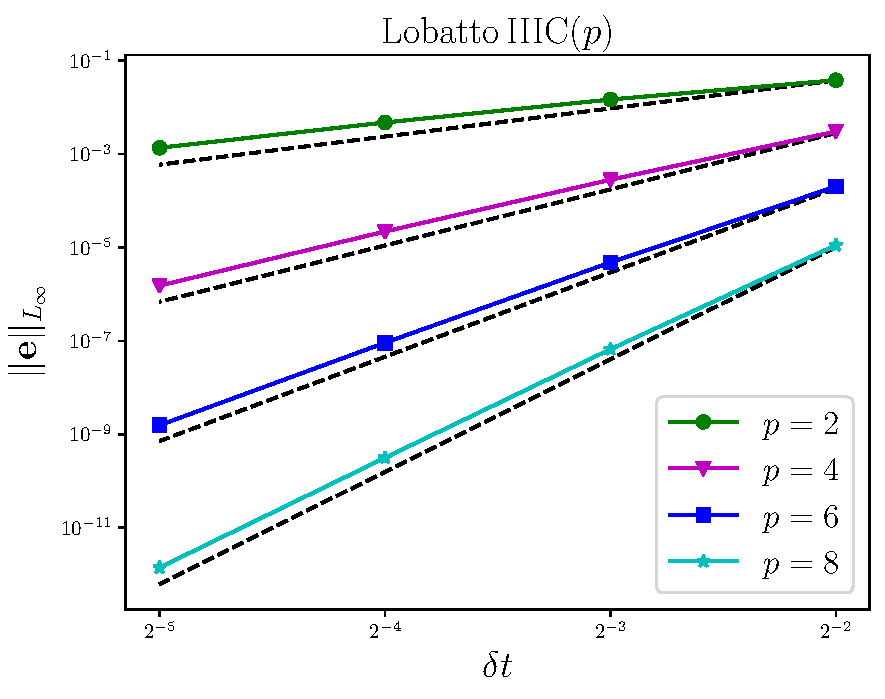
\includegraphics[width = 0.55\textwidth]{figures/LobattoIIIC_d2_ex1.pdf}
}
\caption{$L_{\infty}$ errors measured at $t \approx 2$. Theoretically predicted convergence rates of ${\cal O}(p)$ are shown as dashed black lines.
\label{fig:errors2D}
}
\end{figure}



\begin{figure}[H]
\centerline{
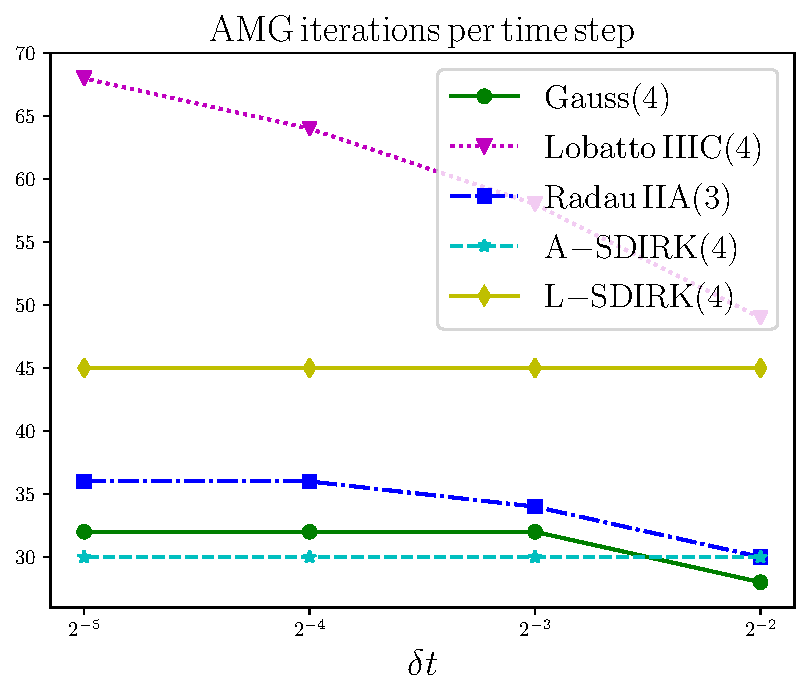
\includegraphics[width = 0.575\textwidth]{figures/amg_iters_14_34_23_-14_4_d2_ex1.pdf}
\quad
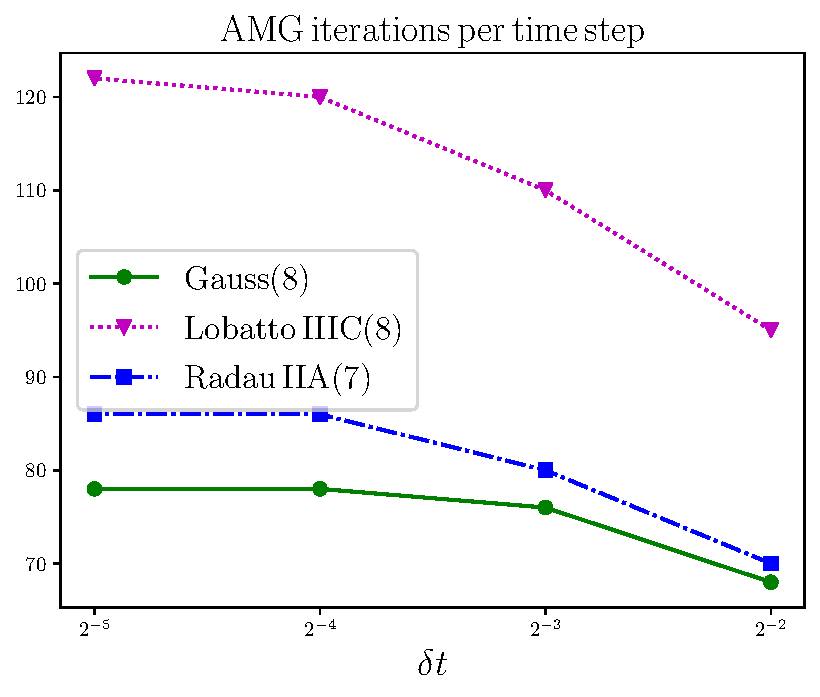
\includegraphics[width = 0.575\textwidth]{figures/amg_iters_18_38_27_d2_ex1.pdf}
}
\centerline{
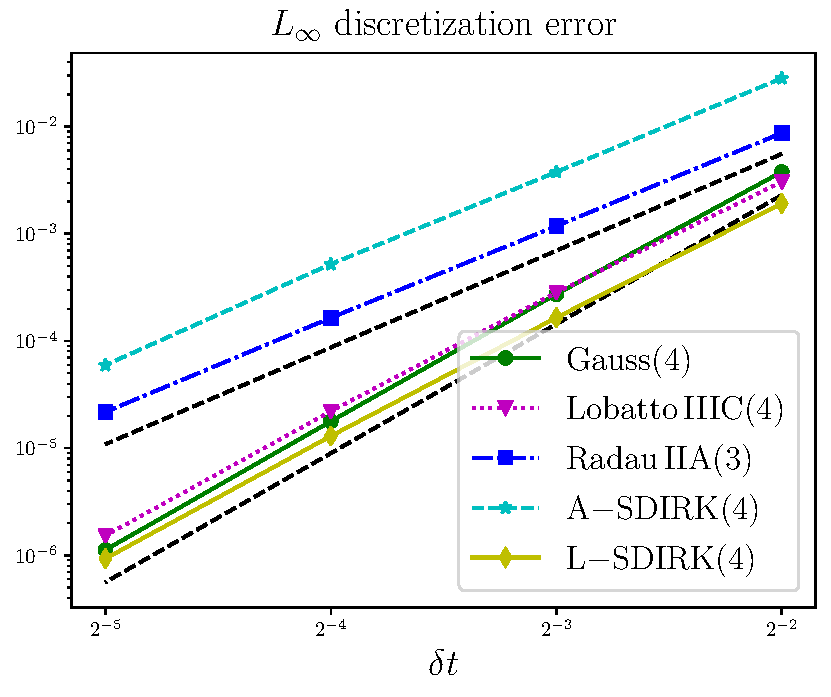
\includegraphics[width = 0.575\textwidth]{figures/errors_iters_14_34_23_-14_4_d2_ex1.pdf}
\quad
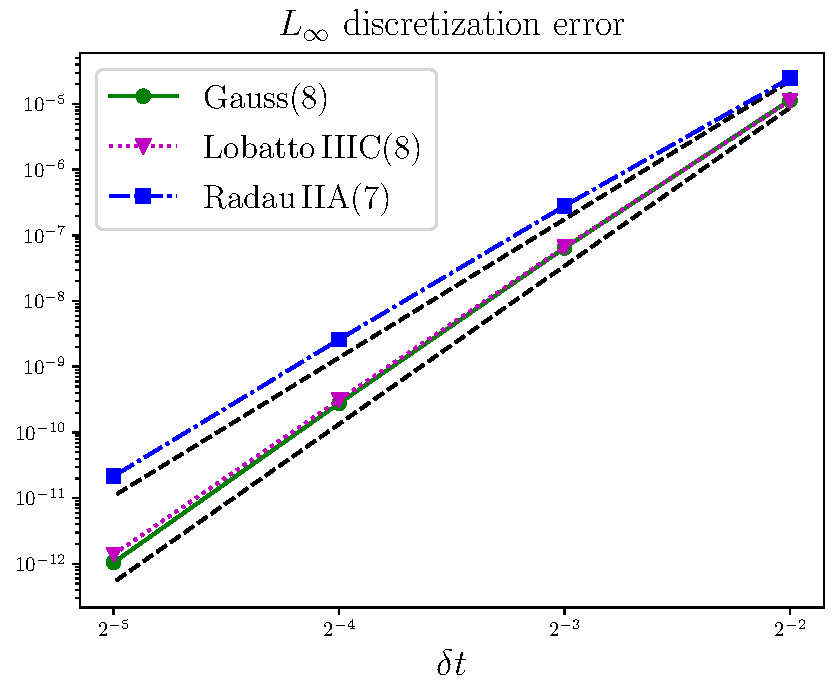
\includegraphics[width = 0.575\textwidth]{figures/errors_iters_18_38_27_d2_ex1.pdf}
}
\caption{Average iterations per time step (data associated with convergence plots in Figure \ref{fig:errors2D}). \textbf{Left:} 4th(ish)-order schemes. \textbf{Right:} 8th(ish)-order schemes. \textbf{Top:} AMG iterations. \textbf{Bottom:} Discretization errors. The systems that AMG is applied to have dimension $n = (16^2, 32^2, 64^2, 128^2)$ for $\delta t = (2^{-2}, 2^{-3}, 2^{-4}, 2^{-5})$. In terms of work done per accuracy, it seems Gauss $<$ Radau IIA $\ll$ Lobatto IIIC. Notice that the error constant for A-SDIRK(4) is much larger that the other 4th-order schemes (bottom left), and convergence appears only $\approx$3rd-order; however, continuing to refine the mesh shows that 4th-order accuracy is obtained eventually (not shown here).
\label{fig:iters2D}
}
\end{figure}




% ------------------------------------------------------------------------------- %
% \bibliographystyle{siamplain}
% \bibliography{refs.bib}

\end{document}



ADJUGATE FORMS, b^T * A0^{-1} * Adj(Ms)
Let M = A0^{-1}, with entries {m_ij}, b = b[b1,...,bs], and xx = spatial operator L

Stiffly accurate RK (b0^TA0^{-1} = [0,...,0,1])
-----------------------------------------------
s = 2
  -m21,
  m11 - xx

s = 3
  -m22 m31 + m21 m32 + m31 xx, 
  m12 m31 - m11 m32 + m32 xx,
  -m12 m21 + m11 m22 - m11 xx - m22 xx + xx^2

s = 4
  m23 m32 m41 - m22 m33 m41 - m23 m31 m42 + m21 m33 m42 + m22 m31 m43 - 
	 m21 m32 m43 + m22 m41 xx + m33 m41 xx - m21 m42 xx - m31 m43 xx - 
	 m41 xx^2,
  -m13 m32 m41 + m12 m33 m41 + m13 m31 m42 - m11 m33 m42 - 
	 m12 m31 m43 + m11 m32 m43 - m12 m41 xx + m11 m42 xx + m33 m42 xx - 
	 m32 m43 xx - m42 xx^2, 
  m13 m22 m41 - m12 m23 m41 - m13 m21 m42 + m11 m23 m42 + m12 m21 m43 - 
	 m11 m22 m43 - m13 m41 xx - m23 m42 xx + m11 m43 xx + m22 m43 xx - 
	 m43 xx^2,
  -m13 m22 m31 + m12 m23 m31 + m13 m21 m32 - m11 m23 m32 - 
	 m12 m21 m33 + m11 m22 m33 + m12 m21 xx - m11 m22 xx + m13 m31 xx + 
	 m23 m32 xx - m11 m33 xx - m22 m33 xx + m11 xx^2 + m22 xx^2 + 
	 m33 xx^2 - xx^3

s = 5
  m24 m33 m42 m51 - m23 m34 m42 m51 - m24 m32 m43 m51 + 
	  m22 m34 m43 m51 + m23 m32 m44 m51 - m22 m33 m44 m51 - 
	  m24 m33 m41 m52 + m23 m34 m41 m52 + m24 m31 m43 m52 - 
	  m21 m34 m43 m52 - m23 m31 m44 m52 + m21 m33 m44 m52 + 
	  m24 m32 m41 m53 - m22 m34 m41 m53 - m24 m31 m42 m53 + 
	  m21 m34 m42 m53 + m22 m31 m44 m53 - m21 m32 m44 m53 - 
	  m23 m32 m41 m54 + m22 m33 m41 m54 + m23 m31 m42 m54 - 
	  m21 m33 m42 m54 - m22 m31 m43 m54 + m21 m32 m43 m54 - 
	  m23 m32 m51 xx + m22 m33 m51 xx - m24 m42 m51 xx - m34 m43 m51 xx + 
	  m22 m44 m51 xx + m33 m44 m51 xx + m23 m31 m52 xx - m21 m33 m52 xx + 
	  m24 m41 m52 xx - m21 m44 m52 xx - m22 m31 m53 xx + m21 m32 m53 xx + 
	  m34 m41 m53 xx - m31 m44 m53 xx - m22 m41 m54 xx - m33 m41 m54 xx + 
	  m21 m42 m54 xx + m31 m43 m54 xx - m22 m51 xx^2 - m33 m51 xx^2 - 
	  m44 m51 xx^2 + m21 m52 xx^2 + m31 m53 xx^2 + m41 m54 xx^2 + 
	  m51 xx^3,
  -m14 m33 m42 m51 + m13 m34 m42 m51 + m14 m32 m43 m51 - 
	  m12 m34 m43 m51 - m13 m32 m44 m51 + m12 m33 m44 m51 + 
	  m14 m33 m41 m52 - m13 m34 m41 m52 - m14 m31 m43 m52 + 
	  m11 m34 m43 m52 + m13 m31 m44 m52 - m11 m33 m44 m52 - 
	  m14 m32 m41 m53 + m12 m34 m41 m53 + m14 m31 m42 m53 - 
	  m11 m34 m42 m53 - m12 m31 m44 m53 + m11 m32 m44 m53 + 
	  m13 m32 m41 m54 - m12 m33 m41 m54 - m13 m31 m42 m54 + 
	  m11 m33 m42 m54 + m12 m31 m43 m54 - m11 m32 m43 m54 + 
	  m13 m32 m51 xx - m12 m33 m51 xx + m14 m42 m51 xx - m12 m44 m51 xx - 
	  m13 m31 m52 xx + m11 m33 m52 xx - m14 m41 m52 xx - m34 m43 m52 xx + 
	  m11 m44 m52 xx + m33 m44 m52 xx + m12 m31 m53 xx - m11 m32 m53 xx + 
	  m34 m42 m53 xx - m32 m44 m53 xx + m12 m41 m54 xx - m11 m42 m54 xx - 
	  m33 m42 m54 xx + m32 m43 m54 xx + m12 m51 xx^2 - m11 m52 xx^2 - 
	  m33 m52 xx^2 - m44 m52 xx^2 + m32 m53 xx^2 + m42 m54 xx^2 + 
	  m52 xx^3, 
  m14 m23 m42 m51 - m13 m24 m42 m51 - m14 m22 m43 m51 + 
	  m12 m24 m43 m51 + m13 m22 m44 m51 - m12 m23 m44 m51 - 
	  m14 m23 m41 m52 + m13 m24 m41 m52 + m14 m21 m43 m52 - 
	  m11 m24 m43 m52 - m13 m21 m44 m52 + m11 m23 m44 m52 + 
	  m14 m22 m41 m53 - m12 m24 m41 m53 - m14 m21 m42 m53 + 
	  m11 m24 m42 m53 + m12 m21 m44 m53 - m11 m22 m44 m53 - 
	  m13 m22 m41 m54 + m12 m23 m41 m54 + m13 m21 m42 m54 - 
	  m11 m23 m42 m54 - m12 m21 m43 m54 + m11 m22 m43 m54 - 
	  m13 m22 m51 xx + m12 m23 m51 xx + m14 m43 m51 xx - m13 m44 m51 xx + 
	  m13 m21 m52 xx - m11 m23 m52 xx + m24 m43 m52 xx - m23 m44 m52 xx - 
	  m12 m21 m53 xx + m11 m22 m53 xx - m14 m41 m53 xx - m24 m42 m53 xx + 
	  m11 m44 m53 xx + m22 m44 m53 xx + m13 m41 m54 xx + m23 m42 m54 xx - 
	  m11 m43 m54 xx - m22 m43 m54 xx + m13 m51 xx^2 + m23 m52 xx^2 - 
	  m11 m53 xx^2 - m22 m53 xx^2 - m44 m53 xx^2 + m43 m54 xx^2 + 
	  m53 xx^3,
  -m14 m23 m32 m51 + m13 m24 m32 m51 + m14 m22 m33 m51 - 
	  m12 m24 m33 m51 - m13 m22 m34 m51 + m12 m23 m34 m51 + 
	  m14 m23 m31 m52 - m13 m24 m31 m52 - m14 m21 m33 m52 + 
	  m11 m24 m33 m52 + m13 m21 m34 m52 - m11 m23 m34 m52 - 
	  m14 m22 m31 m53 + m12 m24 m31 m53 + m14 m21 m32 m53 - 
	  m11 m24 m32 m53 - m12 m21 m34 m53 + m11 m22 m34 m53 + 
	  m13 m22 m31 m54 - m12 m23 m31 m54 - m13 m21 m32 m54 + 
	  m11 m23 m32 m54 + m12 m21 m33 m54 - m11 m22 m33 m54 - 
	  m14 m22 m51 xx + m12 m24 m51 xx - m14 m33 m51 xx + m13 m34 m51 xx + 
	  m14 m21 m52 xx - m11 m24 m52 xx - m24 m33 m52 xx + m23 m34 m52 xx + 
	  m14 m31 m53 xx + m24 m32 m53 xx - m11 m34 m53 xx - m22 m34 m53 xx - 
	  m12 m21 m54 xx + m11 m22 m54 xx - m13 m31 m54 xx - m23 m32 m54 xx + 
	  m11 m33 m54 xx + m22 m33 m54 xx + m14 m51 xx^2 + m24 m52 xx^2 + 
	  m34 m53 xx^2 - m11 m54 xx^2 - m22 m54 xx^2 - m33 m54 xx^2 + 
	  m54 xx^3, 
  m14 m23 m32 m41 - m13 m24 m32 m41 - m14 m22 m33 m41 + 
	  m12 m24 m33 m41 + m13 m22 m34 m41 - m12 m23 m34 m41 - 
	  m14 m23 m31 m42 + m13 m24 m31 m42 + m14 m21 m33 m42 - 
	  m11 m24 m33 m42 - m13 m21 m34 m42 + m11 m23 m34 m42 + 
	  m14 m22 m31 m43 - m12 m24 m31 m43 - m14 m21 m32 m43 + 
	  m11 m24 m32 m43 + m12 m21 m34 m43 - m11 m22 m34 m43 - 
	  m13 m22 m31 m44 + m12 m23 m31 m44 + m13 m21 m32 m44 - 
	  m11 m23 m32 m44 - m12 m21 m33 m44 + m11 m22 m33 m44 + 
	  m13 m22 m31 xx - m12 m23 m31 xx - m13 m21 m32 xx + m11 m23 m32 xx + 
	  m12 m21 m33 xx - m11 m22 m33 xx + m14 m22 m41 xx - m12 m24 m41 xx + 
	  m14 m33 m41 xx - m13 m34 m41 xx - m14 m21 m42 xx + m11 m24 m42 xx + 
	  m24 m33 m42 xx - m23 m34 m42 xx - m14 m31 m43 xx - m24 m32 m43 xx + 
	  m11 m34 m43 xx + m22 m34 m43 xx + m12 m21 m44 xx - m11 m22 m44 xx + 
	  m13 m31 m44 xx + m23 m32 m44 xx - m11 m33 m44 xx - m22 m33 m44 xx - 
	  m12 m21 xx^2 + m11 m22 xx^2 - m13 m31 xx^2 - m23 m32 xx^2 + 
	  m11 m33 xx^2 + m22 m33 xx^2 - m14 m41 xx^2 - m24 m42 xx^2 - 
	  m34 m43 xx^2 + m11 m44 xx^2 + m22 m44 xx^2 + m33 m44 xx^2 - 
	  m11 xx^3 - m22 xx^3 - m33 xx^3 - m44 xx^3 + xx^4

Full implicit RK
----------------
s = 2
  -b1 m12 m21 + b1 m11 m22 - b1 m11 xx - b2 m21 xx,
  -b2 m12 m21 + b2 m11 m22 - b1 m12 xx - b2 m22 xx

s = 3
  -b1 m13 m22 m31 + b1 m12 m23 m31 + b1 m13 m21 m32 - b1 m11 m23 m32 -
     b1 m12 m21 m33 + b1 m11 m22 m33 + b1 m12 m21 xx - b1 m11 m22 xx + 
     b1 m13 m31 xx - b3 m22 m31 xx + b2 m23 m31 xx + b3 m21 m32 xx - 
     b1 m11 m33 xx - b2 m21 m33 xx + b1 m11 xx^2 + b2 m21 xx^2 + 
     b3 m31 xx^2,
  -b2 m13 m22 m31 + b2 m12 m23 m31 + b2 m13 m21 m32 - 
     b2 m11 m23 m32 - b2 m12 m21 m33 + b2 m11 m22 m33 + b2 m12 m21 xx - 
     b2 m11 m22 xx + b3 m12 m31 xx - b3 m11 m32 xx + b1 m13 m32 xx + 
     b2 m23 m32 xx - b1 m12 m33 xx - b2 m22 m33 xx + b1 m12 xx^2 + 
     b2 m22 xx^2 + b3 m32 xx^2,
  -b3 m13 m22 m31 + b3 m12 m23 m31 + 
     b3 m13 m21 m32 - b3 m11 m23 m32 - b3 m12 m21 m33 + b3 m11 m22 m33 +
     b2 m13 m21 xx - b1 m13 m22 xx - b2 m11 m23 xx + b1 m12 m23 xx + 
     b3 m13 m31 xx + b3 m23 m32 xx - b3 m11 m33 xx - b3 m22 m33 xx + 
     b1 m13 xx^2 + b2 m23 xx^2 + b3 m33 xx^2

s = 4
  b1 m14 m23 m32 m41 - b1 m13 m24 m32 m41 - b1 m14 m22 m33 m41 + 
	  b1 m12 m24 m33 m41 + b1 m13 m22 m34 m41 - b1 m12 m23 m34 m41 - 
	  b1 m14 m23 m31 m42 + b1 m13 m24 m31 m42 + b1 m14 m21 m33 m42 - 
	  b1 m11 m24 m33 m42 - b1 m13 m21 m34 m42 + b1 m11 m23 m34 m42 + 
	  b1 m14 m22 m31 m43 - b1 m12 m24 m31 m43 - b1 m14 m21 m32 m43 + 
	  b1 m11 m24 m32 m43 + b1 m12 m21 m34 m43 - b1 m11 m22 m34 m43 - 
	  b1 m13 m22 m31 m44 + b1 m12 m23 m31 m44 + b1 m13 m21 m32 m44 - 
	  b1 m11 m23 m32 m44 - b1 m12 m21 m33 m44 + b1 m11 m22 m33 m44 + 
	  b1 m13 m22 m31 xx - b1 m12 m23 m31 xx - b1 m13 m21 m32 xx + 
	  b1 m11 m23 m32 xx + b1 m12 m21 m33 xx - b1 m11 m22 m33 xx + 
	  b1 m14 m22 m41 xx - b1 m12 m24 m41 xx + b4 m23 m32 m41 xx - 
	  b3 m24 m32 m41 xx + b1 m14 m33 m41 xx - b4 m22 m33 m41 xx + 
	  b2 m24 m33 m41 xx - b1 m13 m34 m41 xx + b3 m22 m34 m41 xx - 
	  b2 m23 m34 m41 xx - b1 m14 m21 m42 xx + b1 m11 m24 m42 xx - 
	  b4 m23 m31 m42 xx + b3 m24 m31 m42 xx + b4 m21 m33 m42 xx - 
	  b3 m21 m34 m42 xx - b1 m14 m31 m43 xx + b4 m22 m31 m43 xx - 
	  b2 m24 m31 m43 xx - b4 m21 m32 m43 xx + b1 m11 m34 m43 xx + 
	  b2 m21 m34 m43 xx + b1 m12 m21 m44 xx - b1 m11 m22 m44 xx + 
	  b1 m13 m31 m44 xx - b3 m22 m31 m44 xx + b2 m23 m31 m44 xx + 
	  b3 m21 m32 m44 xx - b1 m11 m33 m44 xx - b2 m21 m33 m44 xx - 
	  b1 m12 m21 xx^2 + b1 m11 m22 xx^2 - b1 m13 m31 xx^2 + 
	  b3 m22 m31 xx^2 - b2 m23 m31 xx^2 - b3 m21 m32 xx^2 + 
	  b1 m11 m33 xx^2 + b2 m21 m33 xx^2 - b1 m14 m41 xx^2 + 
	  b4 m22 m41 xx^2 - b2 m24 m41 xx^2 + b4 m33 m41 xx^2 - 
	  b3 m34 m41 xx^2 - b4 m21 m42 xx^2 - b4 m31 m43 xx^2 + 
	  b1 m11 m44 xx^2 + b2 m21 m44 xx^2 + b3 m31 m44 xx^2 - b1 m11 xx^3 - 
	  b2 m21 xx^3 - b3 m31 xx^3 - b4 m41 xx^3, 
   b2 m14 m23 m32 m41 - b2 m13 m24 m32 m41 - b2 m14 m22 m33 m41 + 
	  b2 m12 m24 m33 m41 + b2 m13 m22 m34 m41 - b2 m12 m23 m34 m41 - 
	  b2 m14 m23 m31 m42 + b2 m13 m24 m31 m42 + b2 m14 m21 m33 m42 - 
	  b2 m11 m24 m33 m42 - b2 m13 m21 m34 m42 + b2 m11 m23 m34 m42 + 
	  b2 m14 m22 m31 m43 - b2 m12 m24 m31 m43 - b2 m14 m21 m32 m43 + 
	  b2 m11 m24 m32 m43 + b2 m12 m21 m34 m43 - b2 m11 m22 m34 m43 - 
	  b2 m13 m22 m31 m44 + b2 m12 m23 m31 m44 + b2 m13 m21 m32 m44 - 
	  b2 m11 m23 m32 m44 - b2 m12 m21 m33 m44 + b2 m11 m22 m33 m44 + 
	  b2 m13 m22 m31 xx - b2 m12 m23 m31 xx - b2 m13 m21 m32 xx + 
	  b2 m11 m23 m32 xx + b2 m12 m21 m33 xx - b2 m11 m22 m33 xx + 
	  b2 m14 m22 m41 xx - b2 m12 m24 m41 xx - b4 m13 m32 m41 xx + 
	  b3 m14 m32 m41 xx + b4 m12 m33 m41 xx - b3 m12 m34 m41 xx - 
	  b2 m14 m21 m42 xx + b2 m11 m24 m42 xx + b4 m13 m31 m42 xx - 
	  b3 m14 m31 m42 xx - b4 m11 m33 m42 xx + b1 m14 m33 m42 xx + 
	  b2 m24 m33 m42 xx + b3 m11 m34 m42 xx - b1 m13 m34 m42 xx - 
	  b2 m23 m34 m42 xx - b4 m12 m31 m43 xx + b4 m11 m32 m43 xx - 
	  b1 m14 m32 m43 xx - b2 m24 m32 m43 xx + b1 m12 m34 m43 xx + 
	  b2 m22 m34 m43 xx + b2 m12 m21 m44 xx - b2 m11 m22 m44 xx + 
	  b3 m12 m31 m44 xx - b3 m11 m32 m44 xx + b1 m13 m32 m44 xx + 
	  b2 m23 m32 m44 xx - b1 m12 m33 m44 xx - b2 m22 m33 m44 xx - 
	  b2 m12 m21 xx^2 + b2 m11 m22 xx^2 - b3 m12 m31 xx^2 + 
	  b3 m11 m32 xx^2 - b1 m13 m32 xx^2 - b2 m23 m32 xx^2 + 
	  b1 m12 m33 xx^2 + b2 m22 m33 xx^2 - b4 m12 m41 xx^2 + 
	  b4 m11 m42 xx^2 - b1 m14 m42 xx^2 - b2 m24 m42 xx^2 + 
	  b4 m33 m42 xx^2 - b3 m34 m42 xx^2 - b4 m32 m43 xx^2 + 
	  b1 m12 m44 xx^2 + b2 m22 m44 xx^2 + b3 m32 m44 xx^2 - b1 m12 xx^3 - 
	  b2 m22 xx^3 - b3 m32 xx^3 - b4 m42 xx^3, 
   b3 m14 m23 m32 m41 - b3 m13 m24 m32 m41 - b3 m14 m22 m33 m41 + 
	  b3 m12 m24 m33 m41 + b3 m13 m22 m34 m41 - b3 m12 m23 m34 m41 - 
	  b3 m14 m23 m31 m42 + b3 m13 m24 m31 m42 + b3 m14 m21 m33 m42 - 
	  b3 m11 m24 m33 m42 - b3 m13 m21 m34 m42 + b3 m11 m23 m34 m42 + 
	  b3 m14 m22 m31 m43 - b3 m12 m24 m31 m43 - b3 m14 m21 m32 m43 + 
	  b3 m11 m24 m32 m43 + b3 m12 m21 m34 m43 - b3 m11 m22 m34 m43 - 
	  b3 m13 m22 m31 m44 + b3 m12 m23 m31 m44 + b3 m13 m21 m32 m44 - 
	  b3 m11 m23 m32 m44 - b3 m12 m21 m33 m44 + b3 m11 m22 m33 m44 + 
	  b3 m13 m22 m31 xx - b3 m12 m23 m31 xx - b3 m13 m21 m32 xx + 
	  b3 m11 m23 m32 xx + b3 m12 m21 m33 xx - b3 m11 m22 m33 xx + 
	  b4 m13 m22 m41 xx - b4 m12 m23 m41 xx + b2 m14 m23 m41 xx - 
	  b2 m13 m24 m41 xx + b3 m14 m33 m41 xx - b3 m13 m34 m41 xx - 
	  b4 m13 m21 m42 xx + b4 m11 m23 m42 xx - b1 m14 m23 m42 xx + 
	  b1 m13 m24 m42 xx + b3 m24 m33 m42 xx - b3 m23 m34 m42 xx + 
	  b4 m12 m21 m43 xx - b2 m14 m21 m43 xx - b4 m11 m22 m43 xx + 
	  b1 m14 m22 m43 xx + b2 m11 m24 m43 xx - b1 m12 m24 m43 xx - 
	  b3 m14 m31 m43 xx - b3 m24 m32 m43 xx + b3 m11 m34 m43 xx + 
	  b3 m22 m34 m43 xx + b2 m13 m21 m44 xx - b1 m13 m22 m44 xx - 
	  b2 m11 m23 m44 xx + b1 m12 m23 m44 xx + b3 m13 m31 m44 xx + 
	  b3 m23 m32 m44 xx - b3 m11 m33 m44 xx - b3 m22 m33 m44 xx - 
	  b2 m13 m21 xx^2 + b1 m13 m22 xx^2 + b2 m11 m23 xx^2 - 
	  b1 m12 m23 xx^2 - b3 m13 m31 xx^2 - b3 m23 m32 xx^2 + 
	  b3 m11 m33 xx^2 + b3 m22 m33 xx^2 - b4 m13 m41 xx^2 - 
	  b4 m23 m42 xx^2 + b4 m11 m43 xx^2 - b1 m14 m43 xx^2 + 
	  b4 m22 m43 xx^2 - b2 m24 m43 xx^2 - b3 m34 m43 xx^2 + 
	  b1 m13 m44 xx^2 + b2 m23 m44 xx^2 + b3 m33 m44 xx^2 - b1 m13 xx^3 - 
	  b2 m23 xx^3 - b3 m33 xx^3 - b4 m43 xx^3, 
   b4 m14 m23 m32 m41 - b4 m13 m24 m32 m41 - b4 m14 m22 m33 m41 + 
	  b4 m12 m24 m33 m41 + b4 m13 m22 m34 m41 - b4 m12 m23 m34 m41 - 
	  b4 m14 m23 m31 m42 + b4 m13 m24 m31 m42 + b4 m14 m21 m33 m42 - 
	  b4 m11 m24 m33 m42 - b4 m13 m21 m34 m42 + b4 m11 m23 m34 m42 + 
	  b4 m14 m22 m31 m43 - b4 m12 m24 m31 m43 - b4 m14 m21 m32 m43 + 
	  b4 m11 m24 m32 m43 + b4 m12 m21 m34 m43 - b4 m11 m22 m34 m43 - 
	  b4 m13 m22 m31 m44 + b4 m12 m23 m31 m44 + b4 m13 m21 m32 m44 - 
	  b4 m11 m23 m32 m44 - b4 m12 m21 m33 m44 + b4 m11 m22 m33 m44 + 
	  b3 m14 m22 m31 xx - b2 m14 m23 m31 xx - b3 m12 m24 m31 xx + 
	  b2 m13 m24 m31 xx - b3 m14 m21 m32 xx + b1 m14 m23 m32 xx + 
	  b3 m11 m24 m32 xx - b1 m13 m24 m32 xx + b2 m14 m21 m33 xx - 
	  b1 m14 m22 m33 xx - b2 m11 m24 m33 xx + b1 m12 m24 m33 xx + 
	  b3 m12 m21 m34 xx - b2 m13 m21 m34 xx - b3 m11 m22 m34 xx + 
	  b1 m13 m22 m34 xx + b2 m11 m23 m34 xx - b1 m12 m23 m34 xx + 
	  b4 m14 m22 m41 xx - b4 m12 m24 m41 xx + b4 m14 m33 m41 xx - 
	  b4 m13 m34 m41 xx - b4 m14 m21 m42 xx + b4 m11 m24 m42 xx + 
	  b4 m24 m33 m42 xx - b4 m23 m34 m42 xx - b4 m14 m31 m43 xx - 
	  b4 m24 m32 m43 xx + b4 m11 m34 m43 xx + b4 m22 m34 m43 xx + 
	  b4 m12 m21 m44 xx - b4 m11 m22 m44 xx + b4 m13 m31 m44 xx + 
	  b4 m23 m32 m44 xx - b4 m11 m33 m44 xx - b4 m22 m33 m44 xx - 
	  b2 m14 m21 xx^2 + b1 m14 m22 xx^2 + b2 m11 m24 xx^2 - 
	  b1 m12 m24 xx^2 - b3 m14 m31 xx^2 - b3 m24 m32 xx^2 + 
	  b1 m14 m33 xx^2 + b2 m24 m33 xx^2 + b3 m11 m34 xx^2 - 
	  b1 m13 m34 xx^2 + b3 m22 m34 xx^2 - b2 m23 m34 xx^2 - 
	  b4 m14 m41 xx^2 - b4 m24 m42 xx^2 - b4 m34 m43 xx^2 + 
	  b4 m11 m44 xx^2 + b4 m22 m44 xx^2 + b4 m33 m44 xx^2 - b1 m14 xx^3 - 
	  b2 m24 xx^3 - b3 m34 xx^3 - b4 m44 xx^3


Computing A0^{-1} = det(A0)^{-1}Adj(A0)
---------------------------------------
From Wikpedia, The adjugate of A is the n×n matrix whose (i,j) entry is the (j,i)
cofactor of A, (-1)^{i+j} * M_ij, where M_ij is the determinant of the principle
minor of A that comes form deleting rows i and j. Moreover, using the Laplace
formula, computing these minors also yields det(A):
	https://en.wikipedia.org/wiki/Determinant#Laplace's_formula_and_the_adjugate_matrix
I think we should make functions that take an MFEM dense matrix and compute determinants
for a given set of rows and columns, e.g., write the following function for 2,3, and 4
sets of rows/columns:

getMinorDet(DenseMatrix A, int row1, int row2, int col1, int col2)
{
	if (row2 >= A.Height() || col2 >0 A.Width()) {
		error
	}
	return A[row1,col1]*A[row2,col2] - A[row1,col2]*A[row2,col1];
}

Using Laplace formula and adjugate/determinant formula for inverse, these would provide
algebraic inverses for RK tableauxs up to s = 5 with minimal code (could go higher, just
need to add more determinants; 5 stages is probably plenty to start).

Det of 3x3:
-m13 m22 m31 + m12 m23 m31 + m13 m21 m32 - m11 m23 m32 - m12 m21 m33 +
  m11 m22 m33

Det of 4x4:
m14 m23 m32 m41 - m13 m24 m32 m41 - m14 m22 m33 m41 + 
 m12 m24 m33 m41 + m13 m22 m34 m41 - m12 m23 m34 m41 - 
 m14 m23 m31 m42 + m13 m24 m31 m42 + m14 m21 m33 m42 - 
 m11 m24 m33 m42 - m13 m21 m34 m42 + m11 m23 m34 m42 + 
 m14 m22 m31 m43 - m12 m24 m31 m43 - m14 m21 m32 m43 + 
 m11 m24 m32 m43 + m12 m21 m34 m43 - m11 m22 m34 m43 - 
 m13 m22 m31 m44 + m12 m23 m31 m44 + m13 m21 m32 m44 - 
 m11 m23 m32 m44 - m12 m21 m33 m44 + m11 m22 m33 m44


